\documentclass[a4paper]{article}
\usepackage{amsmath}
\usepackage{amsfonts}
\usepackage{amsthm}
\usepackage{amssymb}
\usepackage[english]{babel}
\usepackage{float}
\usepackage{graphicx}
\usepackage{hyperref}
\usepackage[utf8]{inputenc}
\usepackage{listings}
\usepackage{xcolor}
%% \usepackage{subfigure}
\usepackage{pdfpages}
\usepackage{graphicx}
\usepackage{subcaption}
\usepackage{stmaryrd}
\usepackage{a4wide}

\lstset{
  frame=tb,
  language=Python,
  aboveskip=3mm,
  belowskip=3mm,
  showstringspaces=false,
  formfeed=newpage,
  tabsize=4,
  comment=[l]{\#},
  breaklines=true,
  basicstyle=\small
}

\newcommand{\prob}[1]{\mathbb{P}\left(#1\right)}
\newcommand{\expect}[1]{\mathbb{E}\left(#1\right)}
\newcommand{\avg}[1]{\sum_{i=1}^{#1}X_i}
%% \newcommand{\dotp}[2]{\langle #1 + #2 \rangle}
%% \newcommand{\dotp}[2]{\ensuremath{\frac{#1}{#2}}}
\newcommand{\dotpr}[2]{\langle #1,\; #2 \rangle}
\newcommand{\norm}[1]{\left\lVert#1\right\rVert}
\newcommand*{\QEDA}{\hfill\ensuremath{\blacksquare}}%

\title{\vspace{-5cm}ATML Home Assignment 3}
\author{Dmitry Serykh (qwl888)}

\begin{document}
\maketitle
\section{Description}
\label{sec:desc}
In this assignment, I have attempted to reproduce the second experiment from
Thiemann et al for the Ionosphere dataset. I based a portion of my implementation
(including the calculation Jaakkola's heuristic) on my own solution to a similar
exercise from the ML course. I used \emph{python}, \emph{numpy} and SVM solver
from the \emph{sklearn} package. \\\\
I repeated the sin of not performing the experiment multiple times.\\\\
The resulting plot of test losses, running time and bound can be seen
on Figure \ref{plt1}. The source code for my implementation can be found in file
\texttt{experiment.py} in \textbf{handin.zip}.


\begin{figure}
  \centering
  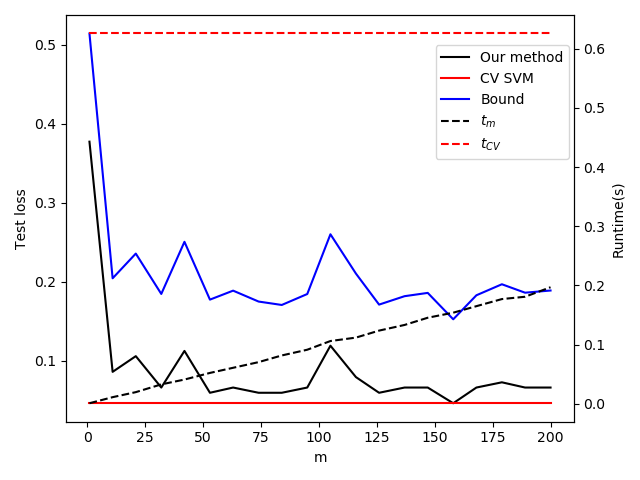
\includegraphics[width=\textwidth]{code/plt1}
  \caption{Comparison of PAC-Bayesian aggregation with RBF kernel SVM
    tuned by cross-validation for the Ionosphere dataset. $n=200$, $r=35$}
  \label{plt1}
\end{figure}

\end{document}

%% \begin{figure}
%%   \centering
%%   \begin{subfigure}[b]{\textwidth}
%%     \centering
%%     \includegraphics[scale=0.8]{handin/plt51}
%%     \caption{Classification of the training set}
%%   \end{subfigure}
%%   \begin{subfigure}[b]{\textwidth}
%%     \centering
%%     \includegraphics[scale=0.8]{handin/plt52}
%%     \caption{Classification of the test set}
%%   \end{subfigure}
%%   \caption{Exercise 5: Logistic Regression Applied to the Datasets}
%%   \label{plt5}
%% \end{figure}

%% \begin{lstlisting}[caption="Calculation of g"]
%% def calc_g(Xs, y, w):
%%     N = np.shape(Xs)[0]
%%     # use matrix X of xs instead of for-loop = much faster
%%     X = np.c_[Xs, np.ones(N)]
%%     num = y.T * X
%%     denum = 1 + np.exp(y * (w @ X.T))
%%     M = num.T/denum
%%     # return mean of each row
%%     return (-1 * np.mean(M, axis=1))
%% \end{lstlisting}
